\scanpage{81}
% archive sheet number: 80
% The typed draft is cancelled by oblique strokes across the page. Marginal pen additions are retained separately.
\deleted{and the induction hypothesis then shows that we have the inequality}
\[
\deleted{\operatorname{long}M/tM\qquad\operatorname{long}M_{\underline{p}_i}\ ,}
\]
\deleted{equality holding if and only if the analogous equalities hold for $M'$ and $M''$, which pqr the induction hypothesis means precisely that b) and c) are \mbox{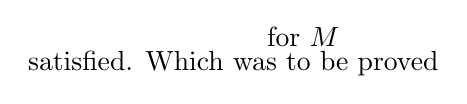
\begin{tikzpicture}[baseline=(base.base)]
\node[inner sep=0] (base) {satisfied. Which was to be proved};
\path (base.north west) -- coordinate[pos=.67] (at) (base.north east);
\node[anchor=south,inner sep=0,yshift=.04cm,xshift=0cm] at (at) {\inserted{for $M$}};
\end{tikzpicture}}}

\deleted{\uline{Corollary} 3. Under the conditions of \mbox{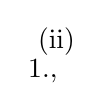
\begin{tikzpicture}[baseline=(base.base)]
\node[inner sep=0] (base) {1.,};
\path (base.north west) -- coordinate[pos=.95] (at) (base.north east);
\node[anchor=south,inner sep=0,yshift=.04cm,xshift=0cm] at (at) {\inserted{(ii)}};
\end{tikzpicture}} suppose that $\operatorname{long}(F/tF)_z$ is equal to 1, then there exists a single irreducible component $S_i$ of $S=\operatorname{supp}F$ passing through $Z$, and if $x$ is its generic point, we have $\operatorname{long}F_x=1$. Moreover, $z$ i s a regular point of \mbox{\begin{tikzpicture}[baseline=(base.base)]
\node[inner sep=0] (base) {$\deleted{S_i}$};
\node[anchor=south west,inner sep=0,xshift=-.18cm,yshift=-.06cm] at (base.north west) {\inserted{$S_{\mathrm{réd}},$}};
\end{tikzpicture}} and $t$ generates the maximal ideal of $\underline{O}_{S_{\mathrm{réd}},z}$.}

\deleted{\uline{Proposition} 4\quad Under the conditions of 1., let $x\quad X$, suppose that $V(t)$ contains no irreducible component $S_i$ of $S=\operatorname{supp}F$ passing through $x$, and that $F/tF$ is reduced at $x$. Then $t$ is $F$-regular at $x$, and $F$ is reduced at $x$.}

\deleted{For the first assertion, the proof is given in 5.6.2. The fact that $F_x$ has no embedded associated prime cycles passing through $x$ is \deleted{a case} then a special case of \unsure{8|6}. below. Remains to prove that the leng\mbox{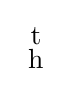
\begin{tikzpicture}[baseline=(base.base)]
\node[inner sep=0] (base) {h};
\path (base.north west) -- coordinate[pos=.5] (at) (base.north east);
\node[anchor=south,inner sep=0,yshift=.04cm,xshift=0cm] at (at) {\inserted{t}};
\end{tikzpicture}}s of $F$ at the maximal generization points of $x$ in $S$ are equal to 1, which is contained in the preceding corollary 3; one could moreover add that the maximal generizations of $x$ in $\operatorname{supp}F/tF$ are regular on $S_{\mathrm{réd}}$ and that $t$ \unsure{generat} the maximal ideal of the local rings of $S_{\mathrm{réd}}$ at these points \ldots}

\deleted{\uline{Proposition} 5. Under the conditions of 1., let $T$ be a prime cycle associated with $F$ (not necessarily maximal), $T'$ a component of $T\quad V(t)$, \deleted{suppose with generic point $x$.} Suppose that $t$ is $F$-regular at the generic point $x$ of $T'$, then \deleted{$T'$ is a} $x\quad\operatorname{Ass}F/tF$.}
\margin{\begin{tikzpicture}[x=1cm,y=1cm]
\node[anchor=base west,rotate=32,inner sep=0] at (0,.50) {\handwritten{Corollary for}};
\node[anchor=base west,rotate=32,inner sep=0] at (.10,0) {\handwritten{$\unsure{x|t}$ \unsure{be|is} $F$ regular\unsure{\mbox{\begin{tikzpicture}[baseline=0cm,x=1cm,y=1cm]
% Two-lobed terminal mark: its value as punctuation or a final letter is unresolved.
\draw[line width=.5pt] (.10,.19) .. controls (.06,.17) and (.03,.13) .. (.03,.10);
\fill (.025,.045) circle (.018cm);
\end{tikzpicture}}}}};
% The grouping stroke stands above and to the right of the slanting note.
\draw[line width=.4pt] (2.82,2.96) -- (3.03,3.02) .. controls (3.00,2.48) and (3.11,1.58) .. (3.00,1.31) -- (3.13,1.25);
\end{tikzpicture}}

\deleted{The proof appears in 8.1.4.}

\deleted{\uline{Corollary} 6. Under the conditions of 1., let $x\quad X$, \deleted{and} suppose that $t$ is $F$-regular at $x$ and that $F/tF$ has no embedded \unsure{associated} prime cyles passing through $x$. Then \mbox{\begin{tikzpicture}[baseline=0cm,x=1cm,y=1cm]
\draw[line width=.5pt] (0,-.25) -- (.17,.22) .. controls (.20,.39) and (.31,.29) .. (.24,.20) -- (.15,.16);
\end{tikzpicture}} the irreducible components of $\operatorname{supp}F/tF$ passing through $x$ are e xactly the irreducible components passing through $X$ of the $S_i\cap V(t)$, where the $S_i$ are the irreducible components of $\operatorname{supp}F=S$}
\margin{\inserted{\handwritten{\shortstack[l]{\mbox{\begin{tikzpicture}[baseline=0cm,x=1cm,y=1cm]
\draw[line width=.5pt] (0,-.25) -- (.17,.22) .. controls (.20,.39) and (.31,.29) .. (.24,.20) -- (.15,.16);
\end{tikzpicture}} $F$ has no\\embedded prime cycles\\\unsure{passing}\\through $x$.}}}}
